\documentclass[12pt,onecolumn,draftclsnofoot]{IEEEtran}

\usepackage[utf8]{inputenc}
\usepackage[T1]{fontenc}
\usepackage[romanian]{babel}
\usepackage{csquotes}
\usepackage{geometry}
\usepackage{setspace}
\usepackage{graphicx}
\usepackage{hyperref}
\usepackage{url}
\usepackage{listings}
\usepackage{xcolor}
\usepackage{longtable}
\usepackage{booktabs}
\usepackage{enumitem}
\usepackage{tikz}
\usepackage{placeins}
\usetikzlibrary{arrows.meta,positioning,shapes.geometric,fit,calc}

\geometry{margin=2.5cm}
\onehalfspacing
\setcounter{tocdepth}{1}
\setcounter{secnumdepth}{2}
\renewcommand{\topfraction}{0.9}
\renewcommand{\textfraction}{0.07}
\renewcommand{\floatpagefraction}{0.85}
\hypersetup{
  colorlinks=true,
  linkcolor=black,
  citecolor=black,
  urlcolor=blue
}

\definecolor{codebg}{RGB}{248,248,248}
\definecolor{codekw}{RGB}{0,92,175}
\definecolor{codecom}{RGB}{0,128,0}

\lstdefinelanguage{Prisma}{
  morekeywords={generator,datasource,model,enum,type,provider,url,env,db,Int,String,DateTime,Boolean,Json,Float,Decimal,Bytes,BigInt,Unsupported,relation,references,fields,onDelete,onUpdate,Cascade,Restrict,SetNull,NoAction,Map,default,updatedAt,id,unique,index,fulltext},
  sensitive=true,
  morecomment=[l]{//},
  morestring=[b]"
}

\lstdefinelanguage{TypeScript}{
  keywords={break,case,catch,class,const,continue,debugger,default,delete,do,else,export,extends,false,finally,for,from,function,if,import,in,instanceof,let,new,null,return,super,switch,this,throw,true,try,typeof,var,void,while,with,yield,async,await,interface,type,implements,public,private,protected,readonly},
  sensitive=true,
  morecomment=[l]{//},
  morecomment=[s]{/*}{*/},
  morestring=[b]",
  morestring=[b]'
}

\lstset{
  basicstyle=\ttfamily\small,
  keywordstyle=\color{codekw}\bfseries,
  commentstyle=\color{codecom}\itshape,
  stringstyle=\color{red!60!black},
  backgroundcolor=\color{codebg},
  frame=single,
  breaklines=true,
  breakatwhitespace=true,
  keepspaces=true,
  xleftmargin=1.5em,
  xrightmargin=0.5em,
  aboveskip=1em,
  belowskip=1em,
  abovecaptionskip=1em,
  belowcaptionskip=1em,
  showstringspaces=false
}

\renewcommand{\contentsname}{Cuprins}

\begin{document}
\begin{titlepage}
  \centering
  {\large UNIVERSITATEA NA\c{T}IONAL\u{A} DE \c{S}TIIN\c{T}\u{A} \c{S}I TEHNOLOGIE POLITEHNICA BUCURE\c{S}TI\par}
  \vspace{0.35cm}
  {\large FACULTATEA DE ELECTRONIC\u{A}, TELECOMUNICA\c{T}II \c{S}I TEHNOLOGIA INFORMA\c{T}IEI\par}
  \vspace{0.35cm}
  {\large PROGRAMUL DE MASTERAT: INGINERIA INFORMA\c{T}IEI \c{S}I A SISTEMELOR DE CALCUL\par}

  \vspace{2.8cm}
  {\Huge \textbf{PROIECT}\par}
  \vspace{0.8cm}
  {\LARGE \textbf{Platform\u{a} educa\c{t}ional\u{a} SQL cu Prisma}\par}
  \vspace{0.3cm}
  {\Large \textbf{Modelare de date, ORM \c{s}i integrare full-stack}\par}

  \vfill
  \begin{minipage}{0.45\textwidth}
    \raggedright
    \textbf{Coordonator \c{s}tiin\c{t}ific:}\\
    S.l. Dr. Ing. Valentin Pupezescu
  \end{minipage}
  \hfill
  \begin{minipage}{0.45\textwidth}
    \raggedleft
    \textbf{Student:}\\
    Ing. Cristi Miloiu\\
    411-IISC
  \end{minipage}

  \vspace{2cm}
  {\large BUCURE\c{S}TI\par}
  {\large 2026\par}
\end{titlepage}

\clearpage
\tableofcontents
\clearpage
\pagenumbering{arabic}

\section{Introducere \c{s}i viziune general\u{a}}

Digitalizarea procesului educa\c{t}ional a condus la apari\c{t}ia unui num\u{a}r semnificativ de platforme de \^{\i}nv\u{a}\c{t}are. Totu\c{s}i, \^{\i}n zona SQL, multe solu\c{t}ii r\u{a}m\^{a}n fie prea teoretice, fie prea pu\c{t}in personalizabile. Proiectul \texttt{sql-learning-platform} porne\c{s}te de la ideea c\u{a} \^{\i}nv\u{a}\c{t}area SQL este eficient\u{a} doar atunci c\^{a}nd utilizatorul execut\u{a} interog\u{a}ri reale pe un context de date controlat, iar progresul este urm\u{a}rit coerent.

Tema proiectului este Prisma, aleas\u{a} nu doar ca utilitar tehnic, ci ca pilon de arhitectur\u{a}. Prisma ofer\u{a} o punte stabil\u{a} \^{\i}ntre modelul rela\c{t}ional (PostgreSQL) \c{s}i codul TypeScript al backend-ului. Prin abordarea \emph{schema-first + generate client}, aplica\c{t}ia ob\c{t}ine consisten\c{t}\u{a} de tipuri, elimin\u{a} o clas\u{a} larg\u{a} de erori runtime \c{s}i simplific\u{a} mentenan\c{t}a pe termen lung.

\subsection{Obiectivele documenta\c{t}iei}
Documenta\c{t}ia are patru obiective principale:
\begin{enumerate}[label=\arabic*)]
  \item descrierea complet\u{a} a arhitecturii software \c{s}i a fluxurilor func\c{t}ionale;
  \item explicarea utiliz\u{a}rii Prisma ca ORM \c{s}i strat de persisten\c{t}\u{a};
  \item justificarea alegerilor de design privind securitatea \c{s}i scalabilitatea;
  \item oferirea unei baze academice solide pentru evaluare \c{s}i extindere ulterioar\u{a}.
\end{enumerate}

\subsection{Contextul tehnologic}
Aplica\c{t}ia este organizat\u{a} \^{\i}n model client-server. Frontend-ul este implementat cu React + Vite, iar backend-ul cu Bun + Elysia. Persisten\c{t}a este asigurat\u{a} de PostgreSQL \c{s}i Prisma. Autentificarea se bazeaz\u{a} pe Google OAuth, iar sesiunile sunt reprezentate prin JWT semnate server-side.

\subsection{Viziune general\u{a} asupra proiectului}
\subsubsection{Scopul aplica\c{t}iei}
Platforma are rolul de a oferi un mediu unificat pentru:
\begin{itemize}
  \item parcurgerea lec\c{t}iilor SQL \^{\i}n ordine pedagogic\u{a};
  \item execu\c{t}ia de comenzi SQL pe o baz\u{a} de date individual\u{a};
  \item urm\u{a}rirea progresului per lec\c{t}ie \c{s}i per utilizator;
  \item separarea strict\u{a} a datelor personale fa\c{t}\u{a} de datele didactice.
\end{itemize}

\subsubsection{Componente principale}
La nivel structural, proiectul con\c{t}ine:
\begin{itemize}
  \item \textbf{client}: interfa\c{t}\u{a} React pentru autentificare, list\u{a} de lec\c{t}ii, lec\c{t}ii individuale \c{s}i set\u{a}ri;
  \item \textbf{server}: API REST construit cu Elysia, responsabil de autentificare, logic\u{a} de business \c{s}i integrarea cu Prisma;
  \item \textbf{prisma schema + migrations}: contractul de date \c{s}i istoricul schimb\u{a}rilor de structur\u{a};
  \item \textbf{docker-compose}: orchestrare pentru rulare local\u{a} sau evaluare.
\end{itemize}

\subsubsection{Rolul central al Prisma}
Prisma joac\u{a} un rol central \^{\i}n:
\begin{enumerate}[label=\alph*)]
  \item definirea modelelor entitate-rela\c{t}ie \^{\i}ntr-un limbaj declarat clar;
  \item generarea unui client TypeScript cu API predictibil;
  \item aplicarea migra\c{t}iilor \^{\i}n medii de dezvoltare \c{s}i produc\c{t}ie;
  \item implementarea opera\c{t}iilor \texttt{find}, \texttt{create}, \texttt{update}, \texttt{upsert}, \texttt{deleteMany} \^{\i}n mod sigur.
\end{enumerate}

\section{Fundamentare teoretic\u{a} \c{s}i analiz\u{a} tehnologic\u{a}}

\subsection{Fundamentare teoretic\u{a}: Prisma ca ORM modern}
\subsubsection{Ce este un ORM}
Un ORM (\emph{Object-Relational Mapping}) permite maparea entit\u{a}\c{t}ilor obiectuale din cod pe tabele rela\c{t}ionale. Beneficiile standard includ reducerea codului boilerplate, consisten\c{t}\u{a} semantic\u{a} \c{s}i abstractizarea dialectelor SQL. Costurile tipice sunt curb\u{a} de \^{\i}nv\u{a}\c{t}are, risc de query-uri ineficiente \^{\i}n lipsa unei model\u{a}ri corecte \c{s}i uneori pierdere de control fin la nivel SQL brut.

\subsubsection{Particularit\u{a}\c{t}i Prisma}
Prisma adreseaz\u{a} limit\u{a}ri istorice ale ORM-urilor tradi\c{t}ionale prin:
\begin{itemize}
  \item \textbf{schema explicit\u{a}}: toate modelele sunt declarate \^{\i}n \texttt{schema.prisma};
  \item \textbf{type safety}: clientul generat folose\c{s}te tipuri stricte \^{\i}n TypeScript;
  \item \textbf{migra\c{t}ii versionate}: schimb\u{a}rile bazei sunt reproducibile;
  \item \textbf{DX ridicat}: syntax\u{a} clar\u{a}, onboarding rapid, integrare bun\u{a} cu editorul.
\end{itemize}

\subsubsection{Prisma ca \enquote{DB layer}}
\^{I}n contextul proiectului curent, Prisma este \enquote{stratul canonic} pentru baza de date aplica\c{t}iei: autentificare utilizator, progres, lec\c{t}ii, metadate ale bazei personale. Chiar dac\u{a} utilizatorul poate executa SQL direct pe propria baz\u{a}, datele nucleu ale platformei r\u{a}m\^{a}n guvernate de Prisma.

\subsection{Compara\c{t}ie Prisma cu alternative ORM}
\subsubsection{Criterii de evaluare}
Compara\c{t}ia dintre Prisma \c{s}i alte op\c{t}iuni uzuale (de exemplu TypeORM, Sequelize, Knex + layer manual) poate fi formulat\u{a} pe urm\u{a}toarele criterii:
\begin{itemize}
  \item claritatea model\u{a}rii datelor;
  \item siguran\c{t}a la compilare \c{s}i ergonomia API-ului;
  \item maturitatea migra\c{t}iilor;
  \item controlul asupra interog\u{a}rilor complexe;
  \item costul de onboarding pentru echipe mici.
\end{itemize}

\subsubsection{Observa\c{t}ii comparative}
Prisma se diferen\c{t}iaz\u{a} prin schema declarativ\u{a} u\c{s}or de citit \c{s}i prin clientul generat care reflect\u{a} fidel modelele. TypeORM ofer\u{a} o abordare \emph{decorator-based} direct \^{\i}n clasele TypeScript, dar poate deveni dificil de men\c{t}inut c\^{a}nd num\u{a}rul de entit\u{a}\c{t}i cre\c{s}te, iar conven\c{t}iile nu sunt standardizate intern. Sequelize este matur, dar orientat istoric pe pattern-uri mai pu\c{t}in stricte tipic pentru TypeScript modern.

Knex, ca query builder, ofer\u{a} control foarte bun la nivel SQL, \^{\i}ns\u{a} necesit\u{a} un efort suplimentar pentru modelare, validare \c{s}i mapare de tipuri. \^{I}n contextul unui proiect educa\c{t}ional full-stack, unde viteza de itera\c{t}ie este critic\u{a}, Prisma ofer\u{a} echilibrul cel mai bun \^{\i}ntre productivitate \c{s}i rigoare.

\subsubsection{Justificarea alegerii finale}
Alegerea Prisma este justificat\u{a} de:
\begin{enumerate}[label=\arabic*)]
  \item integrarea natural\u{a} cu TypeScript;
  \item reducerea num\u{a}rului de defecte legate de schema DB;
  \item migra\c{t}ii transparente \c{s}i u\c{s}or de versionat;
  \item claritate pentru evaluare academic\u{a} \c{s}i colaborare.
\end{enumerate}

\subsection{Analiz\u{a} critic\u{a} a alegerii Prisma}
\subsubsection{Avantaje observate}
Integrarea Prisma \^{\i}n acest proiect aduce:
\begin{itemize}
  \item vitez\u{a} mare de implementare a fluxurilor CRUD;
  \item reducerea bug-urilor de tip mapare c\^{a}mpuri;
  \item evolu\c{t}ie predictibil\u{a} a schemei;
  \item cod mai accesibil pentru echipe mixte (backend + full-stack).
\end{itemize}

\subsubsection{Limit\u{a}ri \c{s}i compromisuri}
Prisma nu elimin\u{a} nevoia de \^{\i}n\c{t}elegere SQL. Pentru optimizare avansat\u{a} este necesar\u{a} analiz\u{a} direct\u{a} a planurilor de execu\c{t}ie. \^{I}n plus, endpoint-urile ce ruleaz\u{a} SQL brut r\u{a}m\^{a}n \^{\i}n afara acoperirii ORM, necesit\^{a}nd guvernan\c{t}\u{a} suplimentar\u{a}.

\subsubsection{Decizie tehnic\u{a} argumentat\u{a}}
Pentru scopul educa\c{t}ional al proiectului, Prisma reprezint\u{a} un echilibru optim \^{\i}ntre productivitate, claritate \c{s}i control. Costurile de adoptare sunt mici, iar beneficiile de consisten\c{t}\u{a} sunt semnificative.

\newpage
\section{Specifica\c{t}ii \c{s}i fluxuri func\c{t}ionale}

\subsection{Fluxuri func\c{t}ionale esen\c{t}iale}
\subsubsection{Autentificare Google + persisten\c{t}\u{a} utilizator}
Endpoint-ul \texttt{/api/auth/google} valideaz\u{a} credentialul \c{s}i ruleaz\u{a}:
\begin{itemize}
  \item \texttt{upsert} \^{\i}n tabela \texttt{User} pe baza \texttt{googleId};
  \item generare JWT cu \texttt{sub=user.id}.
\end{itemize}
Prisma simplific\u{a} semnificativ acest flux: o singur\u{a} opera\c{t}ie acoper\u{a} prima autentificare \c{s}i log\u{a}rile ulterioare.

\begin{figure}[htbp]
  \centering
  \resizebox{0.96\textwidth}{!}{
  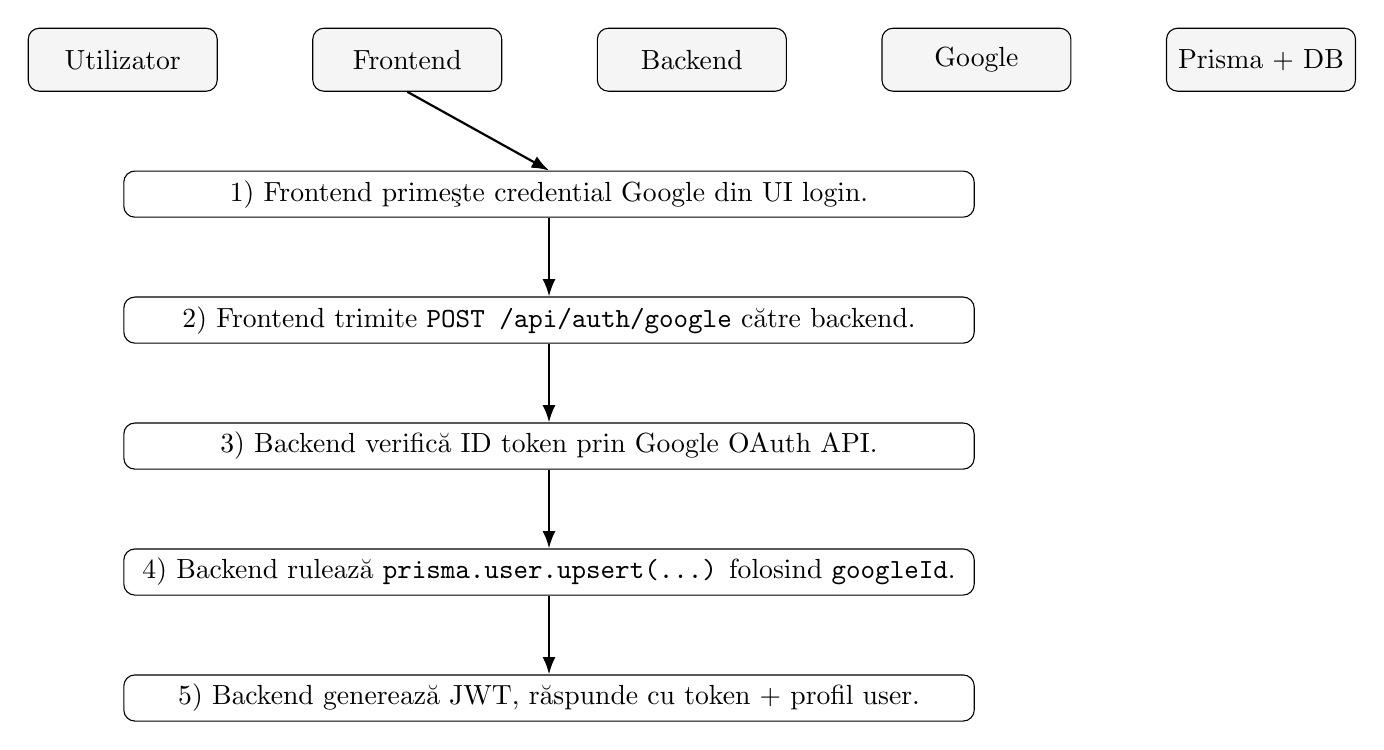
\begin{tikzpicture}[
    node distance=10mm and 12mm,
    lifeline/.style={draw, rounded corners, align=center, minimum width=2.4cm, minimum height=0.8cm, fill=gray!8},
    procstep/.style={draw, rounded corners, align=left, fill=white, minimum width=10.8cm},
    arrow/.style={-{Latex[length=2.2mm]}, thick}
  ]
    \node[lifeline] (u) {Utilizator};
    \node[lifeline, right=of u] (fe) {Frontend};
    \node[lifeline, right=of fe] (be) {Backend};
    \node[lifeline, right=of be] (g) {Google};
    \node[lifeline, right=of g] (db) {Prisma + DB};

    \node[procstep, below=of fe, xshift=1.8cm] (s1) {1) Frontend prime\c{s}te credential Google din UI login.};
    \node[procstep, below=of s1] (s2) {2) Frontend trimite \texttt{POST /api/auth/google} c\u{a}tre backend.};
    \node[procstep, below=of s2] (s3) {3) Backend verific\u{a} ID token prin Google OAuth API.};
    \node[procstep, below=of s3] (s4) {4) Backend ruleaz\u{a} \texttt{prisma.user.upsert(...)} folosind \texttt{googleId}.};
    \node[procstep, below=of s4] (s5) {5) Backend genereaz\u{a} JWT, r\u{a}spunde cu token + profil user.};

    \draw[arrow] (fe.south) -- (s1.north);
    \draw[arrow] (s1.south) -- (s2.north);
    \draw[arrow] (s2.south) -- (s3.north);
    \draw[arrow] (s3.south) -- (s4.north);
    \draw[arrow] (s4.south) -- (s5.north);
  \end{tikzpicture}
  }
  \caption{Secven\c{t}\u{a} de autentificare Google \c{s}i sincronizare utilizator cu Prisma.}
  \label{fig:auth-sequence}
\end{figure}
\FloatBarrier

\subsubsection{Catalog lec\c{t}ii + sincronizare persistent\u{a}}
La accesarea endpoint-urilor de lec\c{t}ii, backend-ul realizeaz\u{a} \texttt{seedCatalog()}:
\begin{enumerate}[label=\alph*)]
  \item \texttt{upsert} pentru fiecare lec\c{t}ie din catalogul static;
  \item \texttt{deleteMany} pentru lec\c{t}ii eliminate din sursa de adev\u{a}r.
\end{enumerate}
Acest mecanism men\c{t}ine consisten\c{t}a \^{\i}ntre defini\c{t}ia didactic\u{a} \c{s}i baza persistent\u{a}.

\subsubsection{Progres utilizator}
La finalizarea unei lec\c{t}ii se execut\u{a} \texttt{upsert} \^{\i}n \texttt{LessonProgress}. Modelul permite reprezentarea separata a:
\begin{itemize}
  \item setup-ului ini\c{t}ial (\texttt{setupAt});
  \item complet\u{a}rii didactice (\texttt{completed}, \texttt{completedAt}).
\end{itemize}

\subsubsection{Gestionarea bazei de date personale}
Conexiunea utilizatorului este:
\begin{enumerate}[label=\arabic*)]
  \item primita prin API;
  \item criptat\u{a} cu AES-GCM pe server;
  \item salvat\u{a} \^{\i}n \texttt{UserDatabase.encryptedUrl};
  \item decriptat\u{a} doar la nevoie pentru opera\c{t}ii live.
\end{enumerate}
\subsection{Specifica\c{t}ii func\c{t}ionale detaliate}
\subsubsection{Use case-uri principale}
Din perspectiv\u{a} didactic\u{a}, sistemul poate fi descris prin urm\u{a}toarele use case-uri:
\begin{enumerate}[label=\arabic*)]
  \item \textbf{Autentificare}: utilizatorul ini\c{t}iaz\u{a} login prin Google \c{s}i prime\c{s}te o sesiune JWT.
  \item \textbf{Vizualizare lec\c{t}ii}: utilizatorul vede lista ordonat\u{a} a lec\c{t}iilor cu starea progresului.
  \item \textbf{Studiu lec\c{t}ie}: utilizatorul acceseaz\u{a} con\c{t}inutul unei lec\c{t}ii \c{s}i eventual setup-ul SQL asociat.
  \item \textbf{Execu\c{t}ie SQL}: utilizatorul ruleaz\u{a} comenzi SQL pe baza sa personal\u{a}.
  \item \textbf{Marcare progres}: utilizatorul marcheaz\u{a} lec\c{t}ia ca finalizat\u{a}.
  \item \textbf{Administrare conexiune DB}: utilizatorul salveaz\u{a} sau genereaz\u{a} o conexiune.
\end{enumerate}

\subsubsection{Actorii sistemului}
Actorii sunt:
\begin{itemize}
  \item \textbf{Utilizator final}: consumatorul platformei educa\c{t}ionale;
  \item \textbf{Server API}: orchestrator fluxuri, autentificare, validare \c{s}i persisten\c{t}\u{a};
  \item \textbf{PostgreSQL aplica\c{t}ie}: stocheaz\u{a} datele interne ale platformei;
  \item \textbf{PostgreSQL utilizator}: mediu practic de rulare SQL;
  \item \textbf{Google Identity}: furnizor extern de identitate.
\end{itemize}

\subsubsection{Cerin\c{t}e func\c{t}ionale sintetice}
\begin{longtable}{p{0.12\textwidth} p{0.8\textwidth}}
\toprule
\textbf{ID} & \textbf{Cerin\c{t}\u{a}} \\
\midrule
F1 & Sistemul trebuie s\u{a} permit\u{a} autentificarea pe baz\u{a} de cont Google \c{s}i s\u{a} creeze automat profilul intern la prima logare. \\
F2 & Sistemul trebuie s\u{a} ofere list\u{a} de lec\c{t}ii cu ordonare deterministic\u{a} \c{s}i statut de progres per utilizator. \\
F3 & Sistemul trebuie s\u{a} permit\u{a} marcarea finaliz\u{a}rii lec\c{t}iilor cu persistarea timestamp-ului. \\
F4 & Sistemul trebuie s\u{a} permit\u{a} configurarea \c{s}i stocarea securizat\u{a} a conexiunii DB a utilizatorului. \\
F5 & Sistemul trebuie s\u{a} permit\u{a} execu\c{t}ia SQL live pe baza utilizatorului \c{s}i afi\c{s}area rezultatului. \\
F6 & Sistemul trebuie s\u{a} permit\u{a} ini\c{t}ializarea dataset-ului de lec\c{t}ie prin scripturi setup idempotente. \\
\bottomrule
\end{longtable}

\section{Arhitectura aplica\c{t}iei}

\subsection{Model arhitectural}
Arhitectura urmeaz\u{a} modelul \emph{Frontend SPA + Backend API + DB}. Clientul comunic\u{a} exclusiv cu API-ul serverului. Serverul:
\begin{itemize}
  \item valideaz\u{a} token-urile;
  \item aplic\u{a} reguli de autorizare;
  \item cite\c{s}te/scrie date prin Prisma;
  \item gestioneaz\u{a} conexiunile dinamice spre baza fiec\u{a}rui utilizator pentru execu\c{t}ie SQL.
\end{itemize}

\subsection{Avantajul separ\u{a}rii responsabilit\u{a}\c{t}ilor}
Separarea \^{\i}ntre \emph{data platform} (Prisma + DB intern) \c{s}i \emph{learning sandbox} (DB utilizator) previne contaminarea datelor, simplific\u{a} auditul de securitate \c{s}i permite extinderea independent\u{a} a fiec\u{a}rei componente.

\subsection{Flux opera\c{t}ional de nivel \^{\i}nalt}
Fluxul tipic este:
\begin{enumerate}[label=\arabic*)]
  \item utilizatorul se autentific\u{a} prin Google OAuth;
  \item serverul verific\u{a} ID token-ul \c{s}i face \texttt{upsert} \^{\i}n tabela \texttt{User};
  \item frontend-ul prime\c{s}te JWT \c{s}i apeleaz\u{a} endpoint-uri protejate;
  \item lec\c{t}iile sunt listate \c{s}i asociate cu progresul;
  \item utilizatorul configureaz\u{a} conexiunea PostgreSQL personal\u{a};
  \item execu\c{t}ia SQL are loc controlat, iar progresul este persistat.
\end{enumerate}

\newpage
\section{Modelarea datelor \c{s}i integrarea Prisma}

\subsection{Modelarea datelor cu Prisma}

\begin{figure}[htbp]
  \centering
  \resizebox{0.96\textwidth}{!}{
  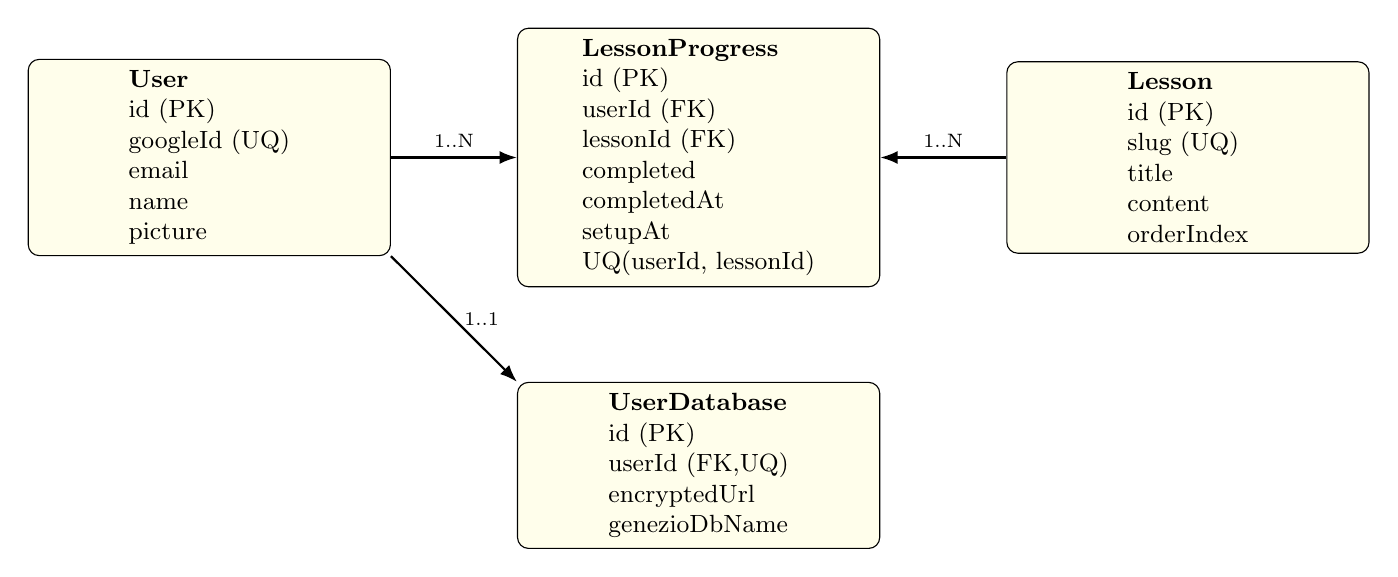
\begin{tikzpicture}[
    node distance=12mm and 16mm,
    ent/.style={draw, rounded corners, align=left, font=\small, fill=yellow!8, inner sep=4pt, minimum width=4.6cm},
    rel/.style={-{Latex[length=2.2mm]}, thick}
  ]
    \node[ent] (user) {\textbf{User}\\id (PK)\\googleId (UQ)\\email\\name\\picture};
    \node[ent, right=of user] (progress) {\textbf{LessonProgress}\\id (PK)\\userId (FK)\\lessonId (FK)\\completed\\completedAt\\setupAt\\UQ(userId, lessonId)};
    \node[ent, right=of progress] (lesson) {\textbf{Lesson}\\id (PK)\\slug (UQ)\\title\\content\\orderIndex};
    \node[ent, below=of progress] (userdb) {\textbf{UserDatabase}\\id (PK)\\userId (FK,UQ)\\encryptedUrl\\genezioDbName};

    \draw[rel] (user.east) -- node[above, font=\scriptsize] {1..N} (progress.west);
    \draw[rel] (lesson.west) -- node[above, font=\scriptsize] {1..N} (progress.east);
    \draw[rel] (user.south east) -- node[right, font=\scriptsize] {1..1} (userdb.north west);
  \end{tikzpicture}
  }
  \caption{Modelul rela\c{t}ional derivat din \texttt{schema.prisma}.}
  \label{fig:prisma-er}
\end{figure}
\FloatBarrier
\subsubsection{Configurare ini\c{t}ial\u{a}}
Fi\c{s}ierul \texttt{schema.prisma} con\c{t}ine generatorul Prisma Client \c{s}i datasource-ul PostgreSQL:
\begin{lstlisting}[language=Prisma,caption={Schema complet\u{a} a bazei de date (schema.prisma)}]
generator client {
  provider = "prisma-client-js"
}

datasource db {
  provider = "postgresql"
  url      = env("DATABASE_URL")
}

model User {
  id        String   @id @default(cuid())
  googleId  String   @unique
  email     String
  name      String?
  picture   String?
  createdAt DateTime @default(now())
  updatedAt DateTime @updatedAt

  lessonsProgress LessonProgress[]
  userDatabase    UserDatabase?
}

model Lesson {
  id          String   @id @default(cuid())
  slug        String   @unique
  title       String
  description String?
  content     String // markdown or HTML
  orderIndex  Int      @default(0)
  createdAt   DateTime @default(now())
  updatedAt   DateTime @updatedAt

  progress LessonProgress[]
}

model LessonProgress {
  id          String    @id @default(cuid())
  userId      String
  lessonId    String
  completed   Boolean   @default(false)
  completedAt DateTime?
  setupAt     DateTime?
  createdAt   DateTime  @default(now())
  updatedAt   DateTime  @updatedAt

  user   User   @relation(fields: [userId], references: [id], onDelete: Cascade)
  lesson Lesson @relation(fields: [lessonId], references: [id], onDelete: Cascade)

  @@unique([userId, lessonId])
  @@index([userId])
  @@index([lessonId])
}

model UserDatabase {
  id             String   @id @default(cuid())
  userId         String   @unique
  encryptedUrl   String?  // null when DB was created via Genezio but URL not returned
  genezioDbName  String?  // e.g. learn-8261d355fb36; one DB per user
  createdAt      DateTime @default(now())
  updatedAt      DateTime @updatedAt

  user User @relation(fields: [userId], references: [id], onDelete: Cascade)

  @@index([userId])
}
\end{lstlisting}

Aceast\u{a} structur\u{a} are dou\u{a} implica\c{t}ii importante:
\begin{itemize}
  \item mediile diferite (dev/prod) sunt controlate din variabile de mediu, nu hardcodate;
  \item clientul ORM este regenarat sincronizat cu schema.
\end{itemize}

\subsubsection{Modelul \texttt{User}}
Entitatea \texttt{User} re\c{t}ine identitatea Google \c{s}i informa\c{t}ii de profil:
\begin{itemize}
  \item \texttt{googleId} este unic \c{s}i sursa primar\u{a} de reconciliere la login;
  \item \texttt{id} este cheie intern\u{a} (\texttt{cuid()}) folosit\u{a} pentru rela\c{t}ii;
  \item rela\c{t}iile cu progresul \c{s}i baza de date a utilizatorului sunt explicite.
\end{itemize}

\subsubsection{Modelul \texttt{Lesson}}
Modelul \texttt{Lesson} exprim\u{a} unitatea didactic\u{a}. C\^{a}mpurile \texttt{slug} \c{s}i \texttt{orderIndex} sunt esen\c{t}iale: primul asigur\u{a} identificare stabil\u{a} \^{\i}n URL, al doilea garanteaz\u{a} ordonarea pedagogic\u{a} independent de ID.

\subsubsection{Modelul \texttt{LessonProgress}}
Acest model capteaz\u{a} starea utilizatorului per lec\c{t}ie. Constr\^{a}ngerea compus\u{a}
\texttt{@@unique([userId, lessonId])} impune unicitatea unei singure \^{\i}nregistr\u{a}ri de progres pentru fiecare pereche utilizator-lec\c{t}ie. Indexurile separate pe \texttt{userId} \c{s}i \texttt{lessonId} optimizeaz\u{a} interog\u{a}ri frecvente.

\subsubsection{Modelul \texttt{UserDatabase}}
Modelul este proiectat pentru a stoca \textbf{doar versiunea criptat\u{a}} a URL-ului de conexiune (\texttt{encryptedUrl}), plus un identificator op\c{t}ional pentru baza generat\u{a} automat. Acest design reduce expunerea accidental\u{a} a credentialelor.

\subsubsection{Integritatea rela\c{t}ional\u{a}}
Toate rela\c{t}iile cheie folosesc \texttt{onDelete: Cascade}. Astfel, eliminarea unui utilizator propag\u{a} automat spre progres \c{s}i metadate asociate, evit\^{a}nd date orfane \c{s}i simplific\^{a}nd mentenan\c{t}a.

\newpage
\subsection{Prisma Client \^{\i}n backend}
\subsubsection{Instan\c{t}iere sigur\u{a}}
Backend-ul folose\c{s}te un singleton Prisma Client cu protec\c{t}ie pentru medii de dezvoltare cu hot reload:
\begin{lstlisting}[language=TypeScript,caption={Singleton Prisma Client}]
const globalForPrisma = globalThis as unknown as { prisma: PrismaClient };

export const prisma =
  globalForPrisma.prisma ??
  new PrismaClient({
    log: process.env.NODE_ENV === "development"
      ? ["query", "error", "warn"]
      : ["error"],
  });

if (process.env.NODE_ENV !== "production") globalForPrisma.prisma = prisma;
\end{lstlisting}

Prin acest pattern se evit\u{a} multiplicarea conexiunilor \^{\i}n sesiuni repetitive de dezvoltare.

\subsubsection{Pattern-uri de acces folosite}
Proiectul utilizeaz\u{a} un set coerent de opera\c{t}ii:
\begin{itemize}
  \item \texttt{upsert} pentru idempotent\u{a} (\texttt{User}, \texttt{Lesson}, \texttt{LessonProgress}, \texttt{UserDatabase});
  \item \texttt{findUnique} pentru acces determinist;
  \item \texttt{findMany} cu \texttt{select} pentru payload minim;
  \item \texttt{deleteMany} pentru sincronizare catalog lec\c{t}ii.
\end{itemize}

\subsubsection{De ce \texttt{upsert} este critic}
\texttt{Upsert} reduce condi\c{t}iile de curs\u{a} \c{s}i elimin\u{a} bifurca\c{t}iile \enquote{dac\u{a} exist\u{a}, altfel creeaz\u{a}}. \^{I}n fluxul login Google, de exemplu, permite actualizarea profilului f\u{a}r\u{a} blocuri separate de cod \c{s}i men\c{t}ine consisten\c{t}a identit\u{a}\c{t}ii.

\newpage
\subsection{Migra\c{t}ii \c{s}i management de schem\u{a}}

\begin{figure}[htbp]
  \centering
  \resizebox{0.96\textwidth}{!}{
  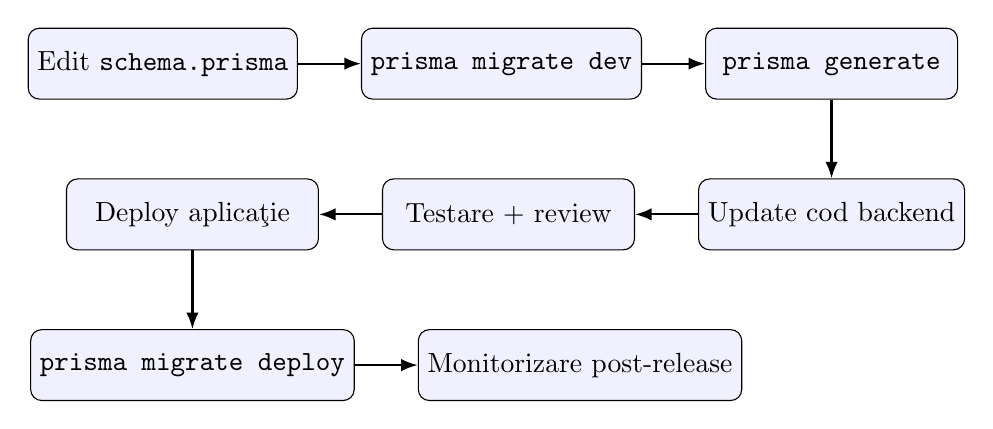
\begin{tikzpicture}[
    node distance=10mm and 8mm,
    st/.style={draw, rounded corners, minimum width=3.2cm, minimum height=0.9cm, align=center, fill=blue!6},
    ar/.style={-{Latex[length=2.1mm]}, thick}
  ]
    \node[st] (a) {Edit \texttt{schema.prisma}};
    \node[st, right=of a] (b) {\texttt{prisma migrate dev}};
    \node[st, right=of b] (c) {\texttt{prisma generate}};
    \node[st, below=of c] (d) {Update cod backend};
    \node[st, left=of d] (e) {Testare + review};
    \node[st, left=of e] (f) {Deploy aplica\c{t}ie};
    \node[st, below=of f] (g) {\texttt{prisma migrate deploy}};
    \node[st, right=of g] (h) {Monitorizare post-release};

    \draw[ar] (a) -- (b);
    \draw[ar] (b) -- (c);
    \draw[ar] (c) -- (d);
    \draw[ar] (d) -- (e);
    \draw[ar] (e) -- (f);
    \draw[ar] (f) -- (g);
    \draw[ar] (g) -- (h);
  \end{tikzpicture}
  }
  \caption{Flux recomandat pentru lifecycle-ul Prisma \^{\i}n proiect.}
  \label{fig:prisma-pipeline}
\end{figure}
\FloatBarrier

\subsubsection{Comenzi de lucru}
Backend-ul expune scripturi explicite:
\begin{itemize}
  \item \texttt{bun run db:generate} -- genereaz\u{a} Prisma Client;
  \item \texttt{bun run db:migrate:dev} -- creeaz\u{a}/aplic\u{a} migra\c{t}ii \^{\i}n dezvoltare;
  \item \texttt{bun run db:migrate} -- aplic\u{a} migra\c{t}ii existente \^{\i}n deployment;
  \item \texttt{bun run db:studio} -- interfa\c{t}\u{a} inspectare date.
\end{itemize}

\subsubsection{Strategie recomandat\u{a}}
Fluxul recomandat pentru o schimbare de model:
\begin{enumerate}[label=\arabic*)]
  \item actualizare \texttt{schema.prisma};
  \item rulare migrare \^{\i}n dev;
  \item validare cu date reale;
  \item commit migrare + schema + cod dependent;
  \item deploy \c{s}i \texttt{migrate deploy}.
\end{enumerate}

\subsubsection{Riscuri \c{s}i mitigare}
Principalele riscuri la migrare sunt: incompatibilit\u{a}\c{t}i de tip, lock pe tabele mari \c{s}i regresii de performan\c{t}\u{a}. Prisma reduce aceste riscuri prin istoricul explicit al migra\c{t}iilor, dar responsabilitatea final\u{a} r\u{a}m\^{a}ne la echipa de dezvoltare (review, backup, testare).

\subsubsection{Sincronizare ORM vs. Migra\c{t}ii generate}
Prisma ofer\u{a} op\c{t}iunea de sincronizare automat\u{a} (prin \texttt{prisma db push}), o func\c{t}ionalitate care aliniaz\u{a} direct baza de date cu schema f\u{a}r\u{a} s\u{a} stocheze istoric. Cu toate acestea, \^{\i}n proiectul curent, aceast\u{a} abordare este strict dezactivat\u{a} pentru ciclurile formale (fiind tolerat\u{a} doar temporar la prototipare iterativ\u{a}). Nu este considerat\u{a} o practic\u{a} bun\u{a} executarea automat\u{a} a primei migr\u{a}ri \^{\i}n produc\c{t}ie, deoarece se pierde vizibilitatea asupra tipurilor de date efective, asupra indec\c{s}ilor s\u{a}pa\c{t}i \c{s}i a clauzelor de constraint generate de baza de date.

\^{I}n schimb, aplica\c{t}ia folose\c{s}te sistemul strict de migra\c{t}ii (\texttt{prisma migrate dev}), care stocheaz\u{a} snapshot-uri exacte de cod SQL. De exemplu, migrarea ini\c{t}ial\u{a} (fi\c{s}ierul \texttt{20250307000000\_init}) cuprinde un cod generat manual/validat de developer:

\begin{lstlisting}[language=SQL,caption={Extras din migrarea ini\c{t}ial\u{a} (Crearea entit\u{a}\c{t}ilor principale)}]
-- CreateTable
CREATE TABLE "User" (
    "id" TEXT NOT NULL,
    "googleId" TEXT NOT NULL,
    "email" TEXT NOT NULL,
    "name" TEXT,
    "picture" TEXT,
    "createdAt" TIMESTAMP(3) NOT NULL DEFAULT CURRENT_TIMESTAMP,
    "updatedAt" TIMESTAMP(3) NOT NULL,

    CONSTRAINT "User_pkey" PRIMARY KEY ("id")
);

-- CreateTable
CREATE TABLE "Lesson" (
    "id" TEXT NOT NULL,
    "slug" TEXT NOT NULL,
    "title" TEXT NOT NULL,
    "description" TEXT,
    "content" TEXT NOT NULL,
    "orderIndex" INTEGER NOT NULL DEFAULT 0,
    "createdAt" TIMESTAMP(3) NOT NULL DEFAULT CURRENT_TIMESTAMP,
    "updatedAt" TIMESTAMP(3) NOT NULL,

    CONSTRAINT "Lesson_pkey" PRIMARY KEY ("id")
);
\end{lstlisting}

Un exemplu puternic al modului \^{\i}n care sistemul de migra\c{t}ii reflect\u{a} evolu\c{t}ia de business a aplica\c{t}iei este modificarea logic\u{a} de "one database per user". \^{I}n acest punct, coloana \texttt{encryptedUrl} a devenit op\c{t}ional\u{a} (\texttt{NULL}) p\u{a}n\u{a} c\u{a}nd infrastructura din spate furnizeaz\u{a} URL-ul, ad\u{a}ug\u{a}ndu-se \c{s}i coloana de nume intern \texttt{genezioDbName}. Aceast\u{a} alterare este salvat\u{a} ireversibil \^{\i}n \texttt{20250307120000\_one\_db\_per\_user}:

\begin{lstlisting}[language=SQL,caption={Evolu\c{t}ia \texttt{UserDatabase} prin migrare incremental\u{a}}]
-- One DB per user: allow row without URL (Genezio created but URL not in response); 
-- store genezio name to avoid creating a second DB
ALTER TABLE "UserDatabase" ADD COLUMN IF NOT EXISTS "genezioDbName" TEXT;
ALTER TABLE "UserDatabase" ALTER COLUMN "encryptedUrl" DROP NOT NULL;
\end{lstlisting}


\newpage
\subsection{Data dictionary extins}
\subsubsection{Tabela \texttt{User}}
\begin{longtable}{p{0.18\textwidth} p{0.14\textwidth} p{0.5\textwidth}}
\toprule
\textbf{C\^{a}mp} & \textbf{Tip} & \textbf{Semnifica\c{t}ie} \\
\midrule
\texttt{id} & String (cuid) & Identificator intern platform\u{a}, cheie primar\u{a}. \\
\texttt{googleId} & String & Identificator unic furnizat de Google Identity. \\
\texttt{email} & String & Email utilizator, folosit \c{s}i \^{\i}n token payload. \\
\texttt{name} & String? & Nume afi\c{s}at \^{\i}n UI (op\c{t}ional). \\
\texttt{picture} & String? & URL avatar Google (op\c{t}ional). \\
\texttt{createdAt} & DateTime & Moment creare cont intern. \\
\texttt{updatedAt} & DateTime & Ultima actualizare automata. \\
\bottomrule
\end{longtable}

\subsubsection{Tabela \texttt{Lesson}}
\begin{longtable}{p{0.18\textwidth} p{0.14\textwidth} p{0.5\textwidth}}
\toprule
\textbf{C\^{a}mp} & \textbf{Tip} & \textbf{Semnifica\c{t}ie} \\
\midrule
\texttt{id} & String (cuid) & Cheie primar\u{a} intern\u{a}. \\
\texttt{slug} & String & Identificator semantic, unic \^{\i}n API \c{s}i rutare UI. \\
\texttt{title} & String & Titlu lec\c{t}ie. \\
\texttt{description} & String? & Rezumat scurt pentru lista lec\c{t}iilor. \\
\texttt{content} & String & Con\c{t}inut principal (markdown/HTML). \\
\texttt{orderIndex} & Int & Pozi\c{t}ie \^{\i}n secven\c{t}a didactic\u{a}. \\
\texttt{createdAt}, \texttt{updatedAt} & DateTime & Audit temporal minimal. \\
\bottomrule
\end{longtable}

\subsubsection{Tabela \texttt{LessonProgress}}
\begin{longtable}{p{0.18\textwidth} p{0.14\textwidth} p{0.5\textwidth}}
\toprule
\textbf{C\^{a}mp} & \textbf{Tip} & \textbf{Semnifica\c{t}ie} \\
\midrule
\texttt{id} & String (cuid) & Cheie primar\u{a}. \\
\texttt{userId} & String & FK spre \texttt{User}. \\
\texttt{lessonId} & String & FK spre \texttt{Lesson}. \\
\texttt{completed} & Boolean & Flag finalizare lec\c{t}ie. \\
\texttt{completedAt} & DateTime? & Timestamp finalizare. \\
\texttt{setupAt} & DateTime? & Timestamp setup dataset lec\c{t}ie. \\
\bottomrule
\end{longtable}

\newpage
\subsubsection{Tabela \texttt{UserDatabase}}
\begin{longtable}{p{0.18\textwidth} p{0.14\textwidth} p{0.5\textwidth}}
\toprule
\textbf{C\^{a}mp} & \textbf{Tip} & \textbf{Semnifica\c{t}ie} \\
\midrule
\texttt{id} & String (cuid) & Cheie primar\u{a}. \\
\texttt{userId} & String & FK unic spre \texttt{User}. \\
\texttt{encryptedUrl} & String? & URL conexiune criptat AES-GCM. \\
\texttt{genezioDbName} & String? & Nume DB creat\u{a} din API extern. \\
\texttt{createdAt}, \texttt{updatedAt} & DateTime & Metadate temporale. \\
\bottomrule
\end{longtable}

\subsection{Prisma \^{\i}n profunzime: internals, decizii \c{s}i pattern-uri}
\subsubsection{Feature-uri Prisma folosite efectiv \^{\i}n proiect}
Pentru a ancora documenta\c{t}ia \^{\i}n implementarea real\u{a} din \texttt{sql-learning-platform}, mai jos sunt func\c{t}ionalit\u{a}\c{t}ile Prisma utilizate direct \^{\i}n codul backend:

\begin{longtable}{p{0.28\textwidth} p{0.62\textwidth}}
\toprule
\textbf{Feature Prisma folosit} & \textbf{Cum este folosit \^{\i}n proiect} \\
\midrule
\texttt{schema.prisma} (\texttt{generator} + \texttt{datasource}) &
Define\c{s}te contractul de date \c{s}i conectarea la PostgreSQL prin \texttt{DATABASE\_URL}. \\
\texttt{model} + rela\c{t}ii (\texttt{@relation}) &
Modelele \texttt{User}, \texttt{Lesson}, \texttt{LessonProgress}, \texttt{UserDatabase} descriu domeniul aplica\c{t}iei \c{s}i leg\u{a}turile dintre entit\u{a}\c{t}i. \\
Constr\^{a}ngeri (\texttt{@unique}, \texttt{@@unique}) &
\texttt{googleId} este unic, iar progresul este garantat unic pe perechea \texttt{(userId, lessonId)}. \\
Indexuri (\texttt{@@index}) &
Accelereaz\u{a} interog\u{a}rile frecvente pe \texttt{lessonProgress} \c{s}i \texttt{userDatabase}. \\
\texttt{onDelete: Cascade} &
Asigur\u{a} cur\u{a}\c{t}area automata a datelor dependente la \c{s}tergeri de entit\u{a}\c{t}i p\u{a}rinte. \\
\texttt{findUnique} &
Folosit pentru acces determinist la utilizator, lec\c{t}ii, progres, configura\c{t}ie DB utilizator. \\
\texttt{findMany} &
Folosit pentru listarea lec\c{t}iilor \c{s}i progresului, cu selectarea controlat\u{a} a c\^{a}mpurilor. \\
\texttt{upsert} &
Folosit intensiv pentru login idempotent, seed lec\c{t}ii, progres lec\c{t}ii, salvare conexiune DB utilizator. \\
\texttt{deleteMany} &
Sincronizeaz\u{a} catalogul persistent cu sursa de adev\u{a}r (\texttt{LESSON\_CATALOG}). \\
\texttt{select} &
Reduce payload-ul trimis c\u{a}tre client (\^{\i}n special \^{\i}n list\u{a}ri). \\
Prisma Client singleton &
Evit\u{a} proliferarea conexiunilor \^{\i}n development (\emph{hot reload safe pattern}). \\
Migra\c{t}ii Prisma &
Gestionate cu \texttt{prisma migrate dev} \c{s}i \texttt{prisma migrate deploy}. \\
\bottomrule
\end{longtable}

\subsubsection{Feature-uri \enquote{related} (nefolosite direct, dar recomandate)}
Urm\u{a}toarele capabilit\u{a}\c{t}i nu sunt nucleare \^{\i}n implementarea curent\u{a}, dar sunt foarte relevante pentru versiuni viitoare:
\begin{itemize}
  \item \texttt{\$transaction} pentru fluxuri multi-mutare strict atomice;
  \item Prisma middleware/extensii pentru audit \c{s}i policies centralizate;
  \item query profiling mai avansat \c{s}i instrumentare runtime;
  \item read replicas \c{s}i optimiz\u{a}ri pentru trafic ridicat.
\end{itemize}

\subsubsection{Interpretare practic\u{a}: ce este \textit{must-have} vs \textit{nice-to-have}}
Pentru acest proiect, \textbf{must-have} sunt deja implementate: modelare, rela\c{t}ii, constr\^{a}ngeri, \texttt{upsert}, \texttt{find*}, migra\c{t}ii \c{s}i singleton client. Elementele \textbf{nice-to-have} sunt cele \enquote{related}, utile mai ales la extindere pe volum mai mare sau cerin\c{t}e opera\c{t}ionale stricte.

\subsubsection{Modelul conceptual Prisma}
Prisma poate fi privit ca un lan\c{t} \enquote{schema $\rightarrow$ client generat $\rightarrow$ query SQL executat}. Pentru un proiect ca \texttt{sql-learning-platform}, acest lan\c{t} aduce un avantaj major: fiecare schimbare din modelul de date propag\u{a} explicit \^{\i}n cod, iar compilatorul TypeScript semnaleaz\u{a} devreme zonele afectate.

La nivel practic, modelul conceptual se traduce astfel:
\begin{enumerate}[label=\arabic*)]
  \item \textbf{Definire structur\u{a}} \^{\i}n \texttt{schema.prisma};
  \item \textbf{Migrare} pentru a sincroniza PostgreSQL cu noua versiune;
  \item \textbf{Generare client} pentru API-ul type-safe;
  \item \textbf{Consum controlat} \^{\i}n rute backend.
\end{enumerate}

\subsubsection{Anatomia unei interog\u{a}ri Prisma}
O interogare Prisma trece prin mai multe etape:
\begin{itemize}
  \item validare shape input \^{\i}n runtime + tipuri la compilare;
  \item transformare \^{\i}n reprezentare intern\u{a} de query;
  \item generare SQL specific dialectului PostgreSQL;
  \item mapare rezultat SQL \^{\i}n obiecte JS/TS.
\end{itemize}

Aceast\u{a} conduct\u{a} explic\u{a} de ce erori comune (c\^{a}mp gre\c{s}it, include/select invalid) sunt prinse mai devreme dec\^{a}t \^{\i}ntr-un strat SQL manual.

\subsubsection{De ce schema actual\u{a} este bine adaptat\u{a} proiectului}
Schema existent\u{a} este minimal\u{a}, dar bine normalizat\u{a} pentru domeniul educa\c{t}ional:
\begin{itemize}
  \item \texttt{User} gestioneaz\u{a} identitatea;
  \item \texttt{Lesson} stocheaz\u{a} obiectul educa\c{t}ional;
  \item \texttt{LessonProgress} modeleaz\u{a} rela\c{t}ia many-to-many cu stare;
  \item \texttt{UserDatabase} separ\u{a} metadatele conexiunii personale.
\end{itemize}

Din punct de vedere al proiect\u{a}rii, cea mai important\u{a} decizie este \texttt{@@unique([userId, lessonId])}. Aceasta encodeaz\u{a} direct regula de business \enquote{un singur progres per utilizator per lec\c{t}ie}, prevenind inconsisten\c{t}e chiar \c{s}i sub concuren\c{t}\u{a}.

\subsubsection{Pattern-ul \texttt{upsert} ca mecanism de consisten\c{t}\u{a}}
Proiectul utilizeaz\u{a} \texttt{upsert} \^{\i}n mai multe fluxuri. Tehnic, \texttt{upsert} are 3 avantaje:
\begin{enumerate}[label=\alph*)]
  \item reduce num\u{a}rul de round-trip-uri DB;
  \item evit\u{a} ramuri \texttt{if (exists) ... else ...} vulnerabile la race condition;
  \item concentreaz\u{a} regula de sincronizare \^{\i}ntr-un singur punct de cod.
\end{enumerate}

Exemplu relevant din proiect:
\begin{lstlisting}[language=TypeScript,caption={Upsert robust pentru progres}]
await prisma.lessonProgress.upsert({
  where: { userId_lessonId: { userId, lessonId: lesson.id } },
  create: { userId, lessonId: lesson.id, completed: true, completedAt: new Date() },
  update: { completed: true, completedAt: new Date() },
});
\end{lstlisting}

Acest pattern este preferabil \^{\i}n endpoint-uri cu trafic concurent (de exemplu click-uri repetate pe \enquote{Complete lesson}).

\subsubsection{Select vs Include: control pe payload \c{s}i cost}
\texttt{select} \c{s}i \texttt{include} sunt instrumente esen\c{t}iale de optimizare:
\begin{itemize}
  \item \texttt{select} limiteaz\u{a} coloanele returnate \c{s}i reduce payload-ul;
  \item \texttt{include} aduce rela\c{t}ii, dar poate cre\c{s}te semnificativ costul interog\u{a}rii.
\end{itemize}

\^{I}n proiect, folosirea \texttt{select} pentru listing-ul de lec\c{t}ii este decizia corect\u{a}, deoarece UI-ul nu are nevoie de \texttt{content} complet la listare. O extensie recomandat\u{a} este standardizarea acestui principiu la toate endpoint-urile de citire.

\subsubsection{Constr\^{a}ngeri Prisma \c{s}i reguli de business}
Prisma permite exprimarea explicit\u{a} a constr\^{a}ngerilor:
\begin{itemize}
  \item unicitate simpl\u{a} (\texttt{@unique});
  \item unicitate compus\u{a} (\texttt{@@unique});
  \item indexare (\texttt{@@index});
  \item integritate referen\c{t}ial\u{a} (\texttt{@relation} + \texttt{onDelete}).
\end{itemize}

O bun\u{a} practic\u{a} este ca orice regul\u{a} de business stabil\u{a} s\u{a} existe \c{s}i la nivel DB (nu doar \^{\i}n cod). Schema proiectului respect\u{a} deja acest principiu pentru progres.

\newpage
\subsubsection{Migra\c{t}ii: strategie tehnic\u{a} matur\u{a}}
Dincolo de comenzile standard, partea important\u{a} este strategia:
\begin{enumerate}[label=\arabic*)]
  \item \textbf{migra\c{t}ii mici, frecvente}, nu schimb\u{a}ri monolitice;
  \item \textbf{evitarea rename-urilor brute} pe tabele mari \^{\i}n ore de v\^{a}rf;
  \item \textbf{compatibilitate backward temporar\u{a}} \^{\i}n deploy gradual;
  \item \textbf{testare migra\c{t}ie pe copie de date realiste}.
\end{enumerate}

Pentru acest proiect, c\^{a}nd se vor introduce modele noi (\texttt{Quiz}, \texttt{Submission}), recomandarea este deploy \^{\i}n doi pa\c{s}i: mai \^{\i}nt\^{a}i schem\u{a} + cod compatibil vechi/nou, apoi cur\u{a}\c{t}are c\^{a}mpuri dep\u{a}\c{s}ite.

\subsubsection{Tranzac\c{t}ii Prisma: c\^{a}nd trebuie folosite}
De\c{s}i proiectul folose\c{s}te opera\c{t}ii atomice punctuale, o zon\u{a} natural\u{a} de extindere este folosirea \texttt{\$transaction} pentru opera\c{t}ii multi-entitate. Regula simpl\u{a}: dac\u{a} dou\u{a} sau mai multe muta\c{t}ii trebuie s\u{a} reeu\c{s}easc\u{a} \enquote{\^{\i}mpreun\u{a} sau deloc}, atunci tranzac\c{t}ia este obligatorie.

Exemplu propus:
\begin{lstlisting}[language=TypeScript,caption={Pattern tranzac\c{t}ional recomandat}]
await prisma.$transaction(async (tx) => {
  const lesson = await tx.lesson.findUnique({ where: { slug } });
  if (!lesson) throw new Error("Lesson not found");

  await tx.lessonProgress.upsert({
    where: { userId_lessonId: { userId, lessonId: lesson.id } },
    create: { userId, lessonId: lesson.id, setupAt: new Date() },
    update: { setupAt: new Date() },
  });

  await tx.user.update({
    where: { id: userId },
    data: { updatedAt: new Date() },
  });
});
\end{lstlisting}

\subsubsection{Concuren\c{t}\u{a}, idempoten\c{t}\u{a} \c{s}i retry}
\^{I}n sisteme web reale, acelea\c{s}i request-uri pot fi trimise de mai multe ori (retries client, timeout-uri, dublu click). Prisma ajut\u{a}, dar designul endpoint-ului r\u{a}m\^{a}ne esen\c{t}ial:
\begin{itemize}
  \item folosi\c{t}i \texttt{upsert} unde opera\c{t}ia este natural idempotent\u{a};
  \item trata\c{t}i explicit erorile de unicitate (de tip P2002) \c{s}i transforma\c{t}i-le \^{\i}n r\u{a}spunsuri HTTP coerente;
  \item evita\c{t}i pattern-ul \texttt{findFirst -> create} f\u{a}r\u{a} protec\c{t}ie tranzac\c{t}ional\u{a}.
\end{itemize}

\subsubsection{Prisma \c{s}i observabilitate}
Observabilitatea bun\u{a} \^{\i}nseamn\u{a} s\u{a} po\c{t}i r\u{a}spunde la \enquote{de ce este lent endpoint-ul X}. Pentru asta:
\begin{enumerate}[label=\arabic*)]
  \item activa\c{t}i loguri Prisma diferen\c{t}iat dev/prod;
  \item ad\u{a}uga\c{t}i corela\c{t}ie request-id \^{\i}n loguri API;
  \item m\u{a}sura\c{t}i separat timpul de query DB vs logic\u{a} aplica\c{t}ie;
  \item analiza\c{t}i periodic query-urile cele mai lente.
\end{enumerate}

\subsubsection{Conexiuni \c{s}i pooling}
Chiar dac\u{a} proiectul folose\c{s}te singleton Prisma Client, la scalare real\u{a} problema principal\u{a} devine managementul conexiunilor:
\begin{itemize}
  \item prea multe instan\c{t}e server pot satura PostgreSQL;
  \item func\c{t}iile serverless pot crea burst-uri de conexiuni;
  \item lipsa unui pooler (ex. PgBouncer) cre\c{s}te laten\c{t}a sub trafic.
\end{itemize}

Recomandarea pentru versiune de produc\c{t}ie extins\u{a}: utilizare pooling dedicat, limitare concuren\c{t}\u{a} pe endpoint-uri costisitoare, backpressure \c{s}i timeouts stricte.

\subsubsection{Boundary-ul dintre Prisma \c{s}i SQL brut}
Proiectul are inten\c{t}ionat endpoint-uri cu SQL brut pentru scop educa\c{t}ional. Tehnic, este important\u{a} delimitarea:
\begin{itemize}
  \item \textbf{Prisma} pentru datele sistemului (\texttt{User}, \texttt{Lesson}, \texttt{Progress});
  \item \textbf{SQL brut controlat} pentru exerci\c{t}ii pe DB utilizator.
\end{itemize}

Aceast\u{a} separare este corect\u{a}. \^{I}n schimb, pentru a reduce riscuri, se recomand\u{a}: whitelist de comenzi \texttt{SELECT}/\texttt{WITH} \^{\i}n mod \enquote{safe}, timeout query la nivel driver, limit\u{a} de r\^{a}nduri returnate.

\subsubsection{Anti-pattern-uri de evitat \^{\i}n evolu\c{t}ia proiectului}
\begin{enumerate}[label=\arabic*)]
  \item ad\u{a}ugarea de c\^{a}mpuri \enquote{generic JSON} f\u{a}r\u{a} motiv solid;
  \item folosirea excesiv\u{a} a \texttt{include} pe rela\c{t}ii ad\^{a}nci;
  \item endpoint-uri care returneaz\u{a} direct obiecte DB complete;
  \item migra\c{t}ii mari \c{s}i riscante, lansate rar;
  \item lipsa testelor de regresie la schimb\u{a}ri de schem\u{a}.
\end{enumerate}

\newpage
\subsubsection{Checklist tehnic Prisma un release}
\begin{longtable}{p{0.38\textwidth} p{0.52\textwidth}}
\toprule
\textbf{Verificare} & \textbf{Criteriu de acceptare} \\
\midrule
Schema valid\u{a} & \texttt{schema.prisma} compileaz\u{a} \c{s}i clientul se genereaz\u{a} f\u{a}r\u{a} warning-uri critice. \\
Migrare sigur\u{a} & Migra\c{t}ia ruleaz\u{a} pe staging cu date realiste \c{s}i f\u{a}r\u{a} pierdere de integritate. \\
Contract API stabil & Endpoint-urile nu expun c\^{a}mpuri sensibile noi accidental. \\
Performan\c{t}\u{a} & Query-urile nou introduse au laten\c{t}\u{a} acceptabil\u{a} sub sarcin\u{a} de test. \\
Observabilitate & Exist\u{a} loguri suficiente pentru diagnosticul incidentelor post-release. \\
\bottomrule
\end{longtable}

\subsubsection{Concluzie tehnic\u{a} pe Prisma}
Pentru \texttt{sql-learning-platform}, Prisma nu este doar un ORM convenabil, ci mecanismul care formalizeaz\u{a} datele sistemului, reduce complexitatea de dezvoltare \c{s}i ofer\u{a} baz\u{a} pentru evolu\c{t}ie sigur\u{a}. Pe m\u{a}sur\u{a} ce proiectul cre\c{s}te, maturitatea va veni din disciplin\u{a} de migrare, observabilitate \c{s}i utilizarea atent\u{a} a tranzac\c{t}iilor.

\section{Documentarea API-ului backend}

\subsection{Endpoint-uri de autentificare}
\begin{longtable}{p{0.40\textwidth} p{0.1\textwidth} p{0.45\textwidth}}
\toprule
\textbf{Endpoint} & \textbf{Metod\u{a}} & \textbf{Descriere} \\
\midrule
\texttt{/api/auth/google} & POST & Prime\c{s}te credential Google, verific\u{a} token, execut\u{a} upsert \^{\i}n \texttt{User}, returneaz\u{a} JWT + user profile. \\
\texttt{/api/auth/me} & GET & Verific\u{a} JWT \c{s}i returneaz\u{a} profilul curent din baza intern\u{a}. \\
\bottomrule
\end{longtable}

\subsection{Endpoint-uri de lec\c{t}ii}
\begin{longtable}{p{0.40\textwidth} p{0.1\textwidth} p{0.45\textwidth}}
\toprule
\textbf{Endpoint} & \textbf{Metod\u{a}} & \textbf{Descriere} \\
\midrule
\texttt{/api/lessons} & GET & Returneaz\u{a} lec\c{t}iile ordonate plus progresul utilizatorului. \\
\texttt{/api/lessons/:slug} & GET & Returneaz\u{a} detalii lec\c{t}ie + setup meta + progres. \\
\texttt{/api/lessons/:slug/setup} & POST & Ruleaz\u{a} setup SQL de lec\c{t}ie pe DB utilizatorului (op\c{t}ional for\c{t}at). \\
\texttt{/api/lessons/:slug/complete} & POST & Marcheaz\u{a} lec\c{t}ia ca finalizat\u{a}. \\
\bottomrule
\end{longtable}

\subsection{Endpoint-uri user database}
\begin{longtable}{p{0.40\textwidth} p{0.1\textwidth} p{0.45\textwidth}}
\toprule
\textbf{Endpoint} & \textbf{Metod\u{a}} & \textbf{Descriere} \\
\midrule
\texttt{/api/user-db} & GET & Returneaz\u{a} starea configur\u{a}rii DB a utilizatorului. \\
\texttt{/api/user-db} & POST & Prime\c{s}te URL conexiune \c{s}i \^{\i}l salveaz\u{a} criptat. \\
\texttt{/api/user-db/generate} & POST & Creeaz\u{a} DB nou\u{a} prin integrare extern\u{a} \c{s}i salveaz\u{a} metadata. \\
\texttt{/api/user-db/decrypted} & GET & Returneaz\u{a} URL decriptat (util intern controlat). \\
\texttt{/api/user-db/live} & GET & Listeaz\u{a} tabele sau date sample dintr-un tabel specificat. \\
\texttt{/api/user-db/run} & POST & Ruleaz\u{a} SQL brut \c{s}i returneaz\u{a} rezultat tabular. \\
\bottomrule
\end{longtable}

\section{Securitate, performan\c{t}\u{a} \c{s}i riscuri}

\subsection{Securitate \c{s}i protec\c{t}ia datelor}
\subsubsection{Principii aplicate}
Platforma aplic\u{a} principii fundamentale:
\begin{itemize}
  \item minimizarea datelor sensibile persistate;
  \item separarea autentific\u{a}rii de autorizare;
  \item validare input la endpoint-uri;
  \item control CORS prin origine configurabil\u{a}.
\end{itemize}

\subsubsection{Prisma \c{s}i securitatea}
Prisma contribuie la securitate indirect prin:
\begin{itemize}
  \item API type-safe, reduc\^{a}nd erori de mapare;
  \item evitarea SQL dinamic pentru opera\c{t}ii de business;
  \item control centralizat al rela\c{t}iilor \c{s}i constr\^{a}ngerilor.
\end{itemize}

\subsubsection{Zone sensibile}
Exist\u{a} dou\u{a} zone care necesit\u{a} aten\c{t}ie ridicat\u{a}:
\begin{enumerate}[label=\alph*)]
  \item endpoint-ul de rulare SQL liber (\texttt{/api/user-db/run});
  \item endpoint-ul de introspec\c{t}ie live (\texttt{/api/user-db/live}).
\end{enumerate}
Fiind inten\c{t}ionat orientate spre \^{\i}nv\u{a}\c{t}are, aceste endpoint-uri trebuie acompaniate de politici de limitare a impactului (rate limiting, sandboxing, timeout-uri stricte).

\subsection{Performan\c{t}\u{a} \c{s}i scalabilitate}
\subsubsection{Caracteristici curente}
Din perspectiva Prisma, proiectul este eficient pentru volum mic-mediu:
\begin{itemize}
  \item interog\u{a}ri simple cu indexuri relevante;
  \item payload-uri selective prin \texttt{select};
  \item opera\c{t}ii idempotente eficiente.
\end{itemize}

\subsubsection{Poten\c{t}iale optimiz\u{a}ri}
Pentru scalare:
\begin{enumerate}[label=\arabic*)]
  \item paginare la endpoint-ul lec\c{t}iilor;
  \item caching pentru catalog static;
  \item monitorizare query plan PostgreSQL;
  \item eventual\u{a} introducere de read replicas;
  \item pooling robust \^{\i}n deployment distribuit.
\end{enumerate}

\subsubsection{Discu\c{t}ie despre costul ORM}
La scar\u{a} foarte mare, overhead-ul ORM poate deveni relevant. \^{I}n acest proiect, compromisurile sunt favorabile: dezvoltare rapid\u{a}, claritate \c{s}i siguran\c{t}\u{a}. Pentru cazuri punctuale, se poate combina Prisma cu query SQL controlat.

\subsection{Matrice de risc}
\subsubsection{Riscuri tehnice}
\begin{longtable}{p{0.22\textwidth} p{0.18\textwidth} p{0.18\textwidth} p{0.32\textwidth}}
\toprule
\textbf{Risc} & \textbf{Probabilitate} & \textbf{Impact} & \textbf{Mitigare} \\
\midrule
Expunere SQL periculos prin endpoint run & Medie & Ridicat & Validare input, roluri, limitare statement-uri, timeout, audit. \\
Cre\c{s}tere laten\c{t}\u{a} la query-uri neindexate & Medie & Mediu & Revizie indexuri, EXPLAIN ANALYZE, monitorizare. \\
Regresii la schimb\u{a}ri de schem\u{a} & Medie & Ridicat & Migra\c{t}ii testate \^{\i}n staging, backup \^{\i}nainte de deploy. \\
Scurgere accidental\u{a} de secrete \^{\i}n loguri & Sc\u{a}zut\u{a} & Ridicat & Redactare loguri, politici de secret scanning. \\
Dependen\c{t}\u{a} de provider extern OAuth & Medie & Mediu & Retry, fallback UX, cache profil local minimal. \\
\bottomrule
\end{longtable}

\subsubsection{Riscuri organiza\c{t}ionale}
\begin{itemize}
  \item lipsa disciplinei de migrare poate produce deriva schemelor;
  \item lipsa testelor automate reduce viteza sigur\u{a} de evolu\c{t}ie;
  \item rota\c{t}ia secretelor f\u{a}r\u{a} plan poate invalida accesul la date.
\end{itemize}

\section{Concluzii}
Proiectul \texttt{sql-learning-platform} demonstreaz\u{a} c\u{a} Prisma poate fi utilizat eficient \^{\i}n dublu rol: motor de modelare/migrare \c{s}i ORM de produc\c{t}ie pentru un backend TypeScript modern. Prin schema clar\u{a}, opera\c{t}ii idempotente, constr\^{a}ngeri rela\c{t}ionale bine definite \c{s}i integrare direct\u{a} \^{\i}n fluxul API, Prisma asigur\u{a} o funda\c{t}ie robust\u{a} pentru o platform\u{a} educa\c{t}ional\u{a} orientat\u{a} spre date.

Din perspectiva calit\u{a}\c{t}ii software, proiectul atinge obiective importante: consisten\c{t}\u{a} a datelor, securitate a informa\c{t}iilor sensibile, extensibilitate \c{s}i mentenan\c{t}\u{a} facil\u{a}. Exist\u{a} zone ce necesit\u{a} maturizare (monitorizare, rate limiting, testare automata extins\u{a}), \^{\i}ns\u{a} funda\c{t}ia este solid\u{a}, iar alegerea Prisma este justificat\u{a} tehnic \c{s}i pedagogic.

Codul surs\u{a} integral al platformei, incluz\^{a}nd arhitectura frontend, backend \c{s}i schema complet\u{a} Prisma, este disponibil open-source pe GitHub la adresa: \url{https://github.com/cristim67/sql-learning-platform}.

\nocite{*}
\bibliographystyle{IEEEtran}
\bibliography{references}

\newpage
\section*{Anexa A: exemple Prisma din proiect}
\subsection*{A.1 Model simplificat}
\begin{lstlisting}[language=Prisma]
model LessonProgress {
  id          String    @id @default(cuid())
  userId      String
  lessonId    String
  completed   Boolean   @default(false)
  completedAt DateTime?
  setupAt     DateTime?

  user   User   @relation(fields: [userId], references: [id], onDelete: Cascade)
  lesson Lesson @relation(fields: [lessonId], references: [id], onDelete: Cascade)

  @@unique([userId, lessonId])
  @@index([userId])
  @@index([lessonId])
}
\end{lstlisting}

\newpage
\subsection*{A.2 Upsert tipic}
\begin{lstlisting}[language=TypeScript]
await prisma.lessonProgress.upsert({
  where: { userId_lessonId: { userId, lessonId: lesson.id } },
  create: { userId, lessonId: lesson.id, completed: true, completedAt: new Date() },
  update: { completed: true, completedAt: new Date() },
});
\end{lstlisting}

\subsection*{A.3 Verificarea token-ului Google OAuth}
\begin{lstlisting}[language=TypeScript]
const response = await fetch(
  `https://oauth2.googleapis.com/tokeninfo?id_token=${idToken}`
);
const payload = await response.json();

if (!response.ok || payload.aud !== process.env.GOOGLE_CLIENT_ID) {
  throw new Error("Token invalid sau expirat.");
}

// Upsert bazat pe googleId
const user = await prisma.user.upsert({
  where: { googleId: payload.sub },
  update: { name: payload.name, picture: payload.picture },
  create: {
    googleId: payload.sub,
    email: payload.email,
    name: payload.name,
    picture: payload.picture,
  },
});
\end{lstlisting}

\newpage
\section*{Anexa B: Opera\c{t}iuni de persisten\c{t}\u{a} \c{s}i tranzac\c{t}ii}
\subsection*{B.1 Seeding idempotent (Catalog de lec\c{t}ii)}
\begin{lstlisting}[language=TypeScript]
// Sincronizarea catalogului hardcodat cu baza de date Prisma
async function seedCatalog() {
  for (const l of LESSON_CATALOG) {
    await prisma.lesson.upsert({
      where: { slug: l.slug },
      create: { slug: l.slug, title: l.title, content: l.content, orderIndex: l.orderIndex },
      update: { title: l.title, content: l.content, orderIndex: l.orderIndex },
    });
  }
  // Curatare lectii obsolete pastrand integritatea referentiala
  const slugs = LESSON_CATALOG.map((l) => l.slug);
  await prisma.lesson.deleteMany({ where: { slug: { notIn: slugs } } });
}
\end{lstlisting}

\subsection*{B.2 Tranzac\c{t}ii native pe mediul utilizatorului (pg driver)}
\begin{lstlisting}[language=TypeScript]
// Executarea de scripturi DDL pe DB-ul dedicat al utilizatorului folosind pg client
const client = await getUserDbConnection(userId);
await client.connect();
try {
  await client.query("BEGIN"); // start tranzactie nativa
  for (const stmt of def.setupSql) {
    await client.query(stmt);
  }
  await client.query("COMMIT");
} catch (e) {
  await client.query("ROLLBACK");
  throw e;
} finally {
  await client.end();
}
\end{lstlisting}

\newpage
\subsection*{B.2 Tranzac\c{t}ii interactive (\$transaction)}
\begin{lstlisting}[language=TypeScript]
// Crearea userului si a bazei de date asociate intr-un pas atomic
const result = await prisma.$transaction(async (tx) => {
  const newUser = await tx.user.create({
    data: {
      email: "student@example.com",
      googleId: "google-oauth-1234",
      name: "Student"
    }
  });

  const userDb = await tx.userDatabase.create({
    data: {
      userId: newUser.id,
      genezioDbName: `db_${newUser.id}`,
      encryptedUrl: "encrypted_string_aici..."
    }
  });

  return { user: newUser, db: userDb };
});
\end{lstlisting}



\end{document}
